\chapter{帮你上手可删}

听说你对latex使用不熟,下面给你书写一些基本操作

\section{这是章节内一级标题}

\subsection{这是章节内二级标题}

\subsubsection{这是章节内三级标题}


\section{列表}

\subsection{有序列表}

使用enumerate 命令

\begin{enumerate}
    \item 第一点
    \item 第二点
    \item 第三点
\end{enumerate}

\subsection{无序列表}

使用itemize 命令

\begin{itemize}
    \item 巴拉巴拉
    \item 淅沥淅沥
    \item 哗啦哗啦
\end{itemize}


\section{公式}

\subsection{行内公式}

使用美元符号\$将公式圈起来:$\frac{1}{2}mV^2=E_k$;

一段输入转矩$T_{1.in}$,最大功率$P_{\max}$等等

\subsection{行间公式}

如果需要编号,使用begin\{equation\}命令

\begin{equation}
    \alpha=\alpha_0+\frac{L_d-L}{2}
\end{equation}

latex自动为您编号:

\begin{equation}
    d_1\geq 76.6\left( \frac{K\cdot T_1}{\Psi_d^2[\sigma]_{H2}^2}\cdot\frac{\mu+1}{\mu} \right)^{\frac{1}{3}}
\end{equation}

若无需编号,使用双美元\$\$包围:

$$
v=\frac{\pi d n}{60\times 1000}
$$

\subsection{常用符号}

\begin{itemize}
    \item $\cos,\sin,\tan,\ln$:\textbackslash cos,\textbackslash sin,\textbackslash tan,\textbackslash ln(前加反斜杠)
    \item $\cdot$:cdot命令
    \item $\times$:times命令
    \item $x_a^b$:下标\_\{内容\},上标 \^{}\{内容\}
    \item $^{\circ}$:\^{} \{\textbackslash circ\}
    \item $\sqrt{x}$:\textbackslash sqrt命令
    \item $\frac{a}{b}$:分数,\textbackslash frac命令
    \item $P_{\text{许用}}$:汉字,使用\textbackslash text\{\}命令包裹汉字
    \item $\left( \frac{1}{3}\right)$:括号变大符号,使用left,right控制
    \item $\alpha,\beta,\Psi$:希腊字母,请用的时候查阅
    \item $\%$:latex里百分号意味着注释,使用前加上\textbackslash 反斜杠用以转义
\end{itemize}


可以使用网站:https://www.latexlive.com/编辑公式

\section{文献索引}

文献编码全在content/Refrence文件中,我已经写了三个。使用cite命令即可索引,如cite:

根据课设书本\cite{1},结合书本\cite{2}可以得到巴拉巴拉

需要补充的话按照我的格式书写即可

\section{插入图片}

请将图片统一放置在目录figure下,比如我要插入figure下的文件传动简图,我需要:

\begin{figure}[H]  %% H强制图片出现在当前位置
    \centering  %% 居中
    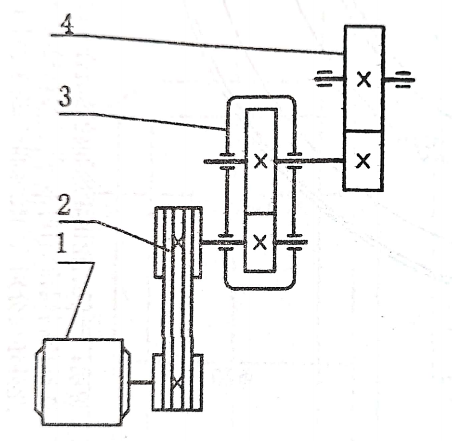
\includegraphics[width=0.5\textwidth]{figure/传动简图.png}
    \caption{传动简图草绘}
    \label{传动简图}
\end{figure}

caption是图片下面的注释,而label是可以用来索引的,比如我索引图片\ref{传动简图},使用ref命令;

可以用width=xx \textbackslash textwidth来设置图像大小

其他图像插入方法自行百度

\section{表格}

这块内容比较复杂。我自己掌握的比较好了,但总体来说还有欠缺;可以随时问我,比如:

% Please add the following required packages to your document preamble:
% \usepackage{graphicx}
\begin{table}[H]
\centering
\caption{总体设计大作业某个表格}
\resizebox{\textwidth}{!}{%
\begin{tabular}{|c|c|c|}
\hline
\textbf{部分名称} & \textbf{部分重量} & \textbf{部分重心位置(离机头)$/kg$} \\ \hline
\textbf{机身} & \textbf{$M_{FUS}=32555.4kg$} & \textbf{$x_{FUS}=\frac{66.18}{2}=33.08m$} \\ \hline
\textbf{机翼} & \textbf{$M_{w}=20572.37kg$} & \textbf{$x_{w}=30.1717m$} \\ \hline
\textbf{水平尾翼} & \textbf{$M_{H}=2042.42kg$} & \textbf{$x_{H}=64.328m$} \\ \hline
\textbf{垂直尾翼} & \textbf{$M_{V}=928.00kg$} & \textbf{$x_{V}=64.263m$} \\ \hline
\textbf{起落装置} & \textbf{$M_{lg}=11792.9kg$} & \textbf{$x_{lg}=x_G$} \\ \hline
\textbf{动力装置} & \textbf{$M_{pow}=22704.2kg$} & \textbf{$x_{pow}=23.8197$} \\ \hline
\textbf{系统和设备} & \textbf{$M_{system}=29723.9kg$} & \textbf{$x_{system}=x_G$} \\ \hline
\textbf{使用项目} & \textbf{$M_{op}=6975kg$} & \textbf{$x_{op}=x_G$} \\ \hline
\textbf{有效载荷} & \textbf{$M_{eff}=33860kg$} & \textbf{$x_{eff}=30.7892m$} \\ \hline
\textbf{燃油} & \textbf{$M_f=79110.7kg$} & \textbf{$x_{f}=x_w=39.1717m$} \\ \hline
\textbf{全集总重与质心位置} & \textbf{$M_G=240264.89kg$} & \textbf{$x_G=m$} \\ \hline
\end{tabular}%
}
\end{table}

同样的可以对表格设置caption和label,一般跟在centering后面;不赘述


可以直接把excel复制到网址https://www.tablesgenerator.com/上,生成latex表格代码